\appendix
\chapter{Algorithm}
\section{Efficient Phase Space Construction}\label{sec:algorithm}
\paragraph*{}
We found that it was possible to analyze the full phase space for all random Boolean networks of size $ N \leq 29 $. However, the computation time needed per realization for the larger networks was on an average machine on the order of several minutes. Thus it would not have been reasonable to use those for statistical purposes. We found $N=14$ to be the size with which we could work for most cases, but if the ensembles had to be larger, we decided to limit ourselves to $N=10$.

\paragraph*{}
Our algorithm is fairly straightforward and easily implementable for other cases than only random Boolean networks. The concept is closely related to building tree-structured graphs since the basins of attraction would actually only be trees if we remove the states that belong to the cycle.

\paragraph*{}
We start by creating a class that holds additional information for every (current) state of the phase space $c$, namely a container that stores which states can lead to it $\{p_1,p_2,\dots,p_k\}$, which one comes in the next time step $n$ and its final attractor's label. We can represent this information for every state visually:

\begin{figure}[h!]
	\centering
		\begin{tikzpicture}[x=1cm, y=1cm]
		\vertex (p1) at (0,2) {$p_1$};
		\vertex (p2) at (0,1) {$p_2$};

		\vertex (p4) at (0,-1) {$p_k$};
		\vertex (c) at (3,0.5) {$c$};
		\vertex (n) at (6,0.5) {$n$};
		
		\draw [->,thick] 
		(p1) edge (c)
		(p2) edge (c)
		(p4) edge (c)
		(c) edge (n);
		\draw (0,0) node {$\vdots$};
		\draw (4,-0.7) node[rectangle,draw] {Attractor label};
		\draw [thick] (3,-0.45) -- (3,0.15);
		
		\end{tikzpicture}
	\par	
\end{figure}

\paragraph*{}
To fill the information in for every state, we have to obey the following steps. Remember that every state can be interpreted as a number. Using this, we begin by choosing the lowest yet not visited state and look at its evolution of the next time step. We can use this to store the next state's information to our current state and the current one is obviously a predecessor of the following one. We use the next state afterward as our current one and repeat the procedure. Thereby we always check if the following state has already been applied with a previous one. At this point, we would stop since it would mean one of two things.

\paragraph*{}
First, we could have reached a cycle and we get to know whether that is the case by looking at the next node attractor label. Because if it does not already belong to an attractor, the only way we could find an existing predecessor for the next time step would be that we have visited in this previous path. The other possibility would be that it already belongs to a basin of attraction.

\paragraph*{}
Either way, we start going backward and apply all the previous nodes with the attractor's label we either have hit on our path or, if we have found just a cycle, give them all a yet unused attractor label. If we have ended up at the state from which we started the path, we can start ones again from the now lowest not visited state. This way, we go through the whole phase space only about two times, one forward and one backward. The information we are interested in can either be collected during the run or afterward by iterating through the states with their full data. If we are interested in the in-degree of the states, the latter option would be the way to go.

\paragraph*{}
There are a few traps one could walk into if not being careful enough. One of them could be to naively implement the backward path so that it stops if there is no previous node anymore. If we initialized on a cycle, this would mean that we get stuck in an infinite loop. But checking if the previous node has an attractor label instead of just assigning it already fixes this.

\paragraph*{}
\chapter{Further Figures}
\section{Statistical Values for Critical Networks}
\begin{figure}[h!]
	\centering
	\begin{subfigure}{\textwidth}
		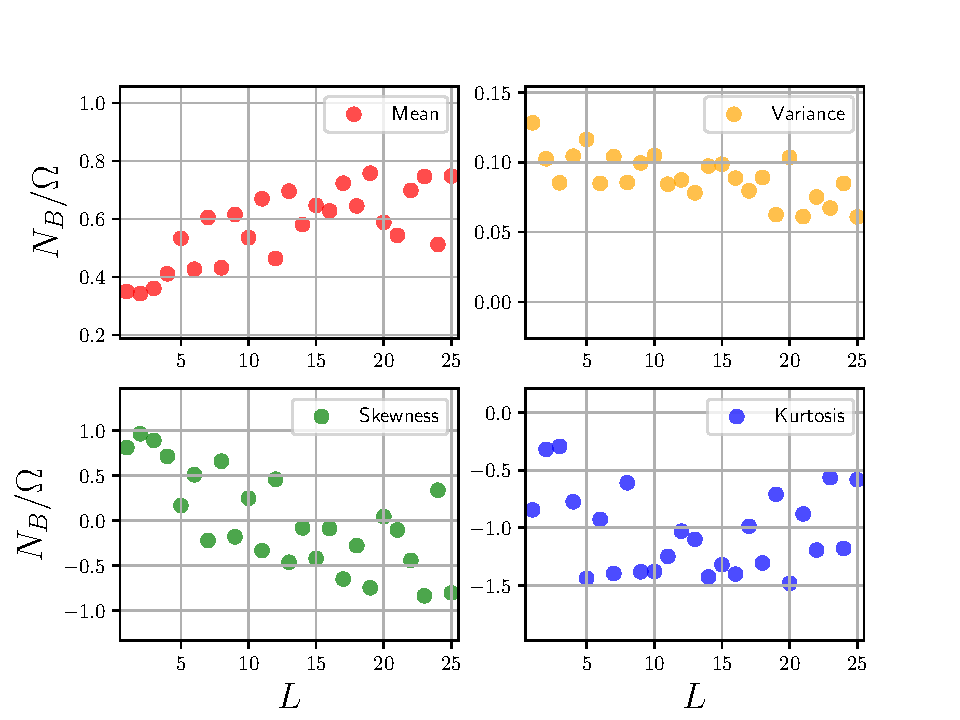
\includegraphics[width=\textwidth]{Plots/mvsk_N10_K2}
	\end{subfigure}
	\caption{Here we provide some statistical values with higher moments of the distributions of the critical networks (see Figure \ref{fig:new_scatter} on the right). This has been one of the first approaches in trying to understand the variations in the basin sizes. Since we could not find any useful information in this plots, we decided to separate them from our main work. So we decided to put them here for the interested reader.}
	\label{fig:statistical_values}
	\par
\end{figure}
\newpage
\section{Additional Plots to Figure \hyperref[fig:basin_sizes_main]{3.4}}
\begin{figure}[h!]
\begin{subfigure}{\textwidth}
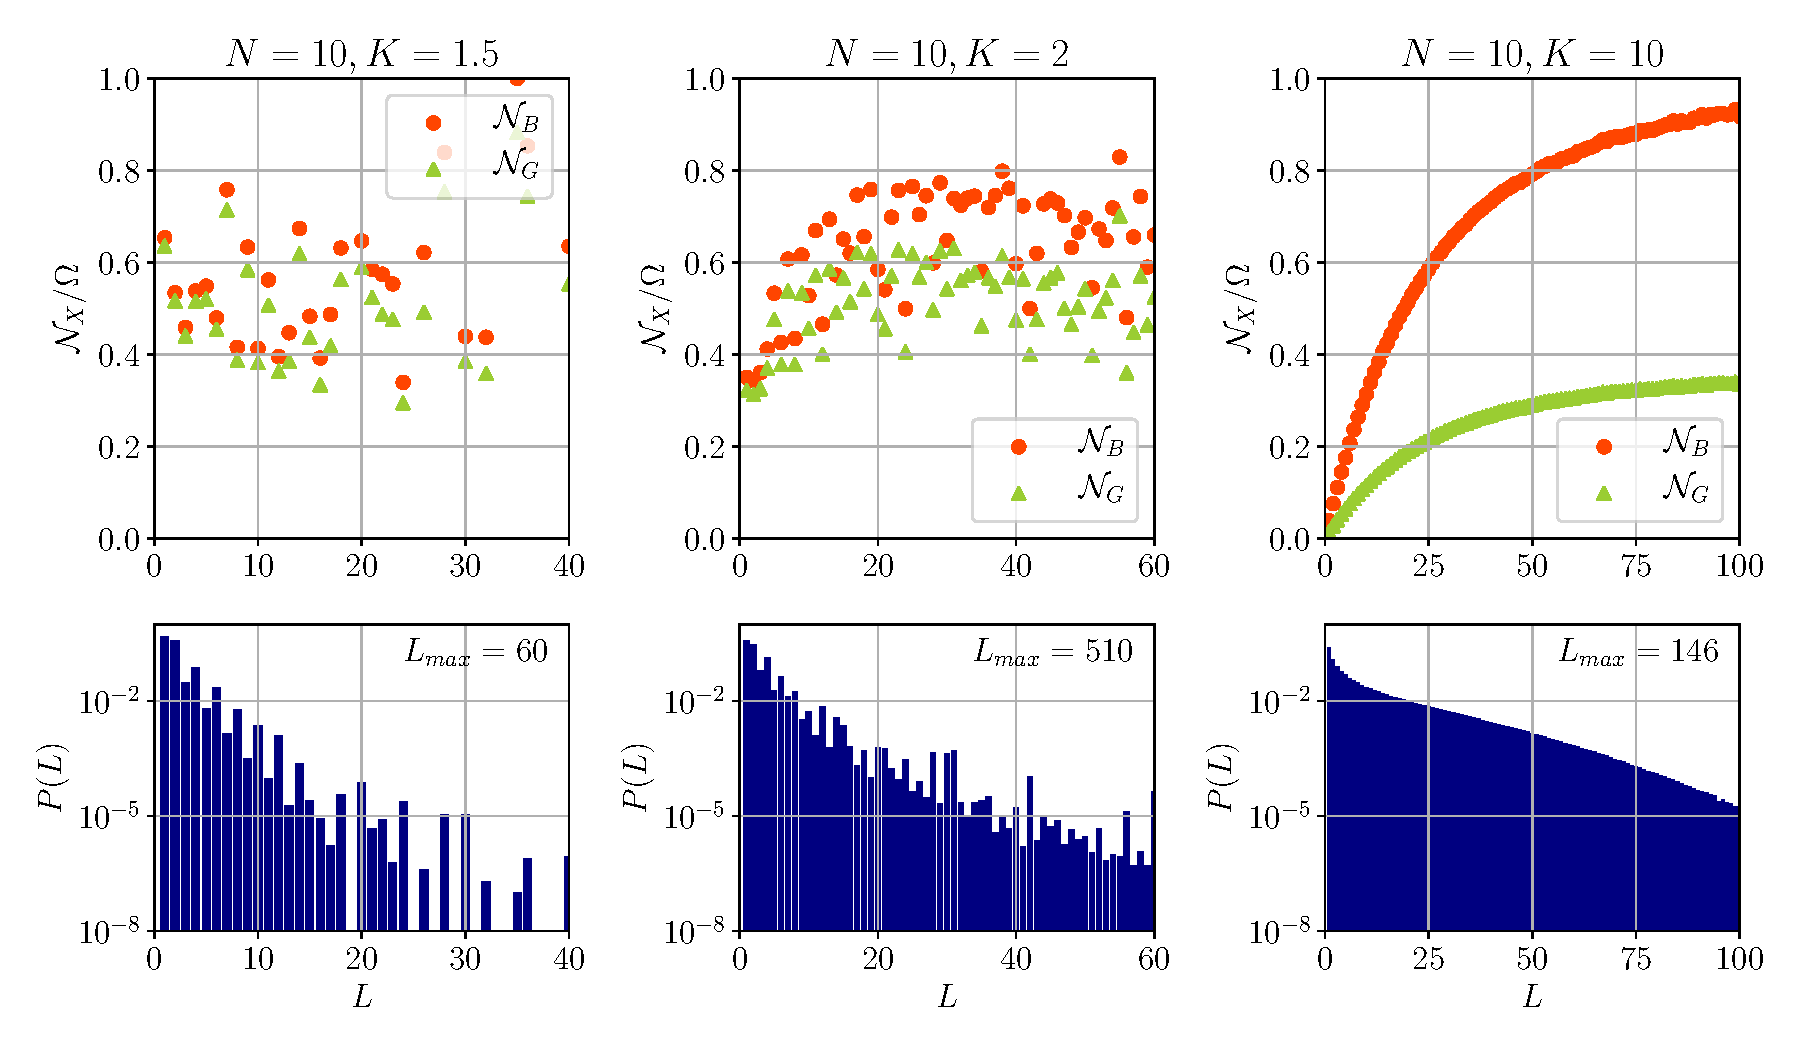
\includegraphics[width=\textwidth]{Plots/basin_sizes_N10}
\end{subfigure}
\begin{subfigure}{\textwidth}
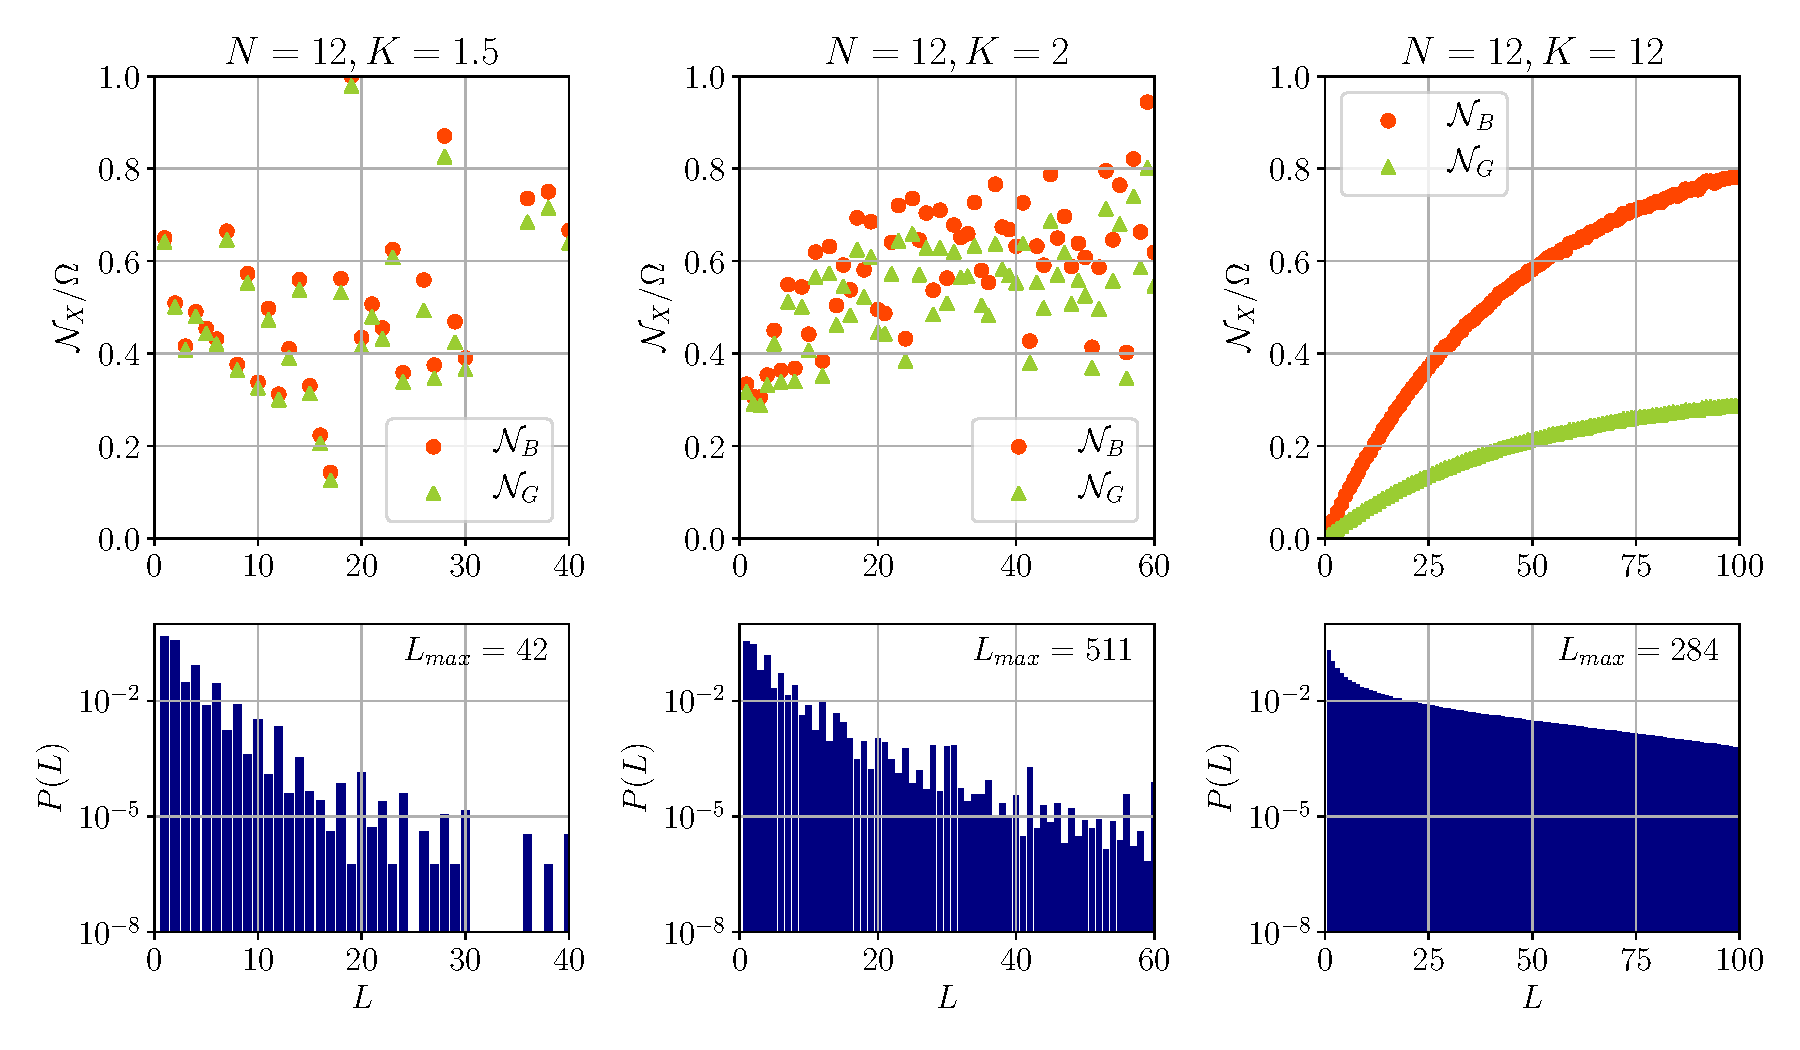
\includegraphics[width=\textwidth]{Plots/basin_sizes_N12}
\end{subfigure}
	\caption{Here we see plots like in Figure \ref{fig:basin_sizes_main}, only now for the sizes $N=10$ and $N=12$. The first were done over $10^7$ realizations and the second over $10^6$. The upper plots show the averaged normalized basins of attraction (orange) and the part that the garden-of-Eden states (green) take up from the whole phase space. Below them we have the probability distribution for attractors with length L to appear.}
	\label{fig:basin_sizes_main_additional_sizes}
\end{figure}

\begin{figure}[h!]
	\begin{subfigure}{\textwidth}
		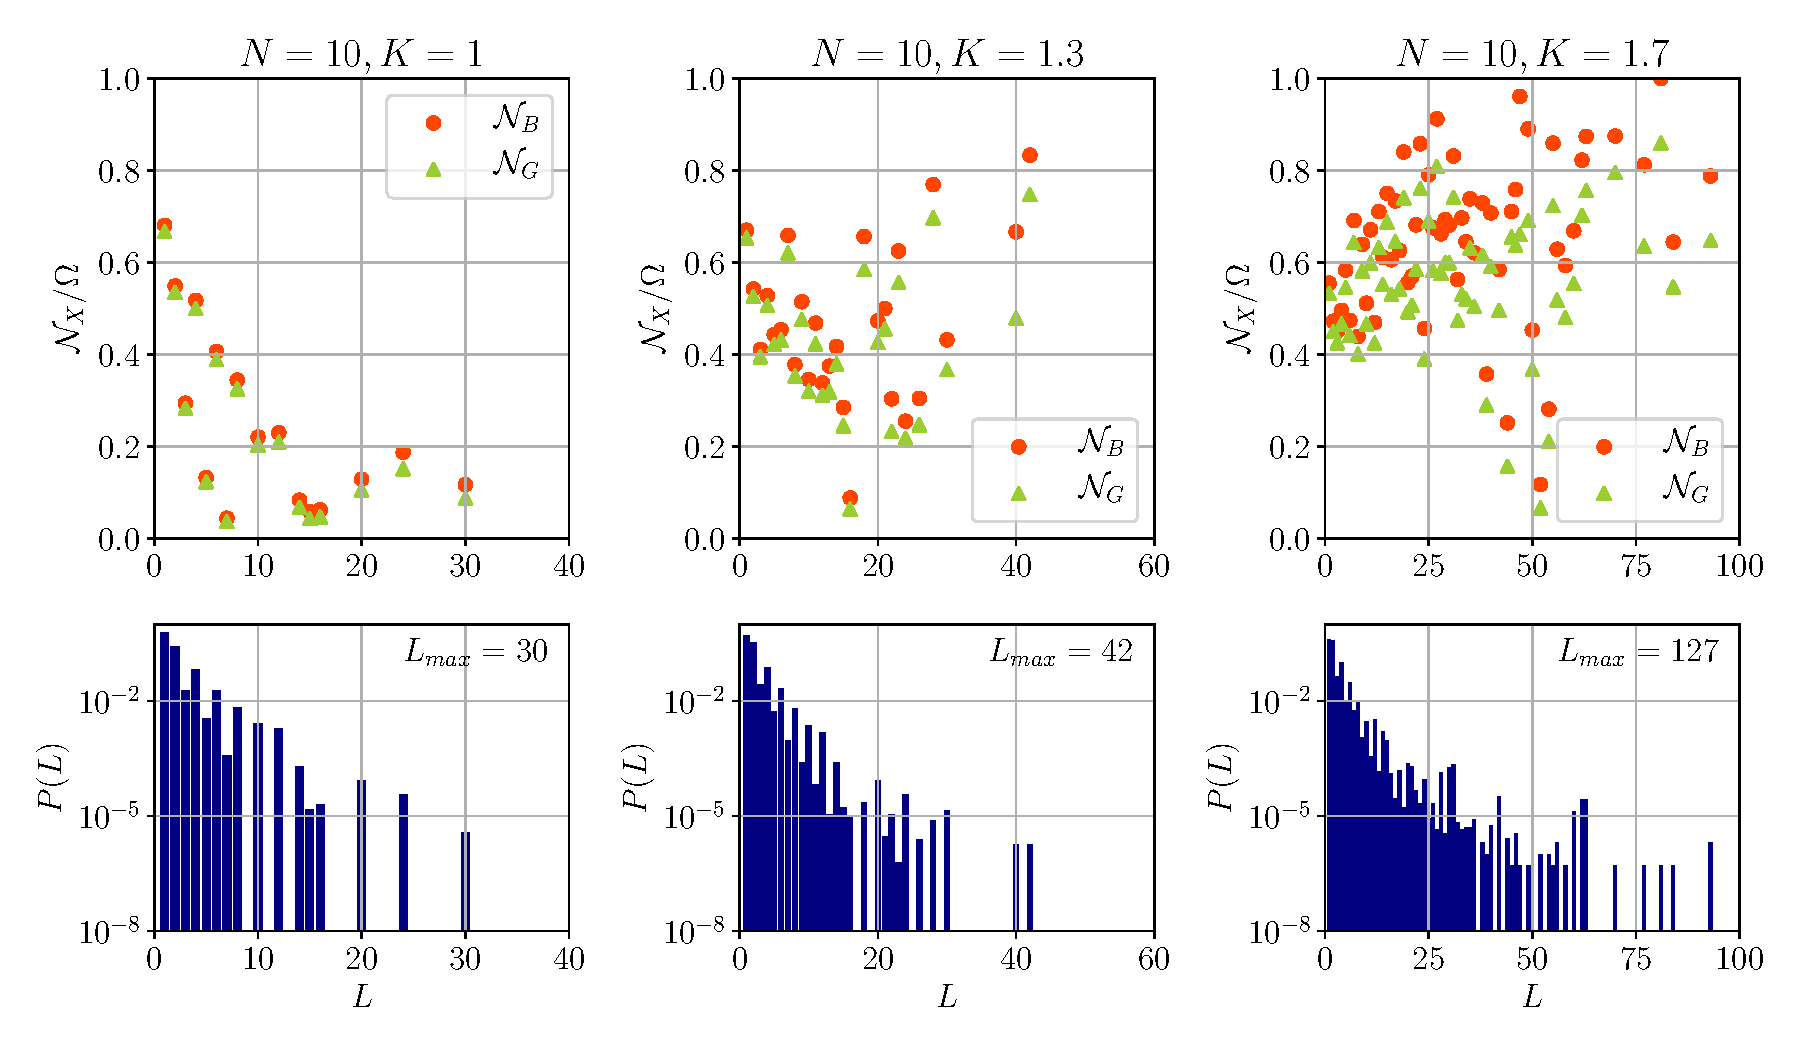
\includegraphics[width=\textwidth]{Plots/basin_sizes_N10_frozen}
	\end{subfigure}
	\begin{subfigure}{\textwidth}
		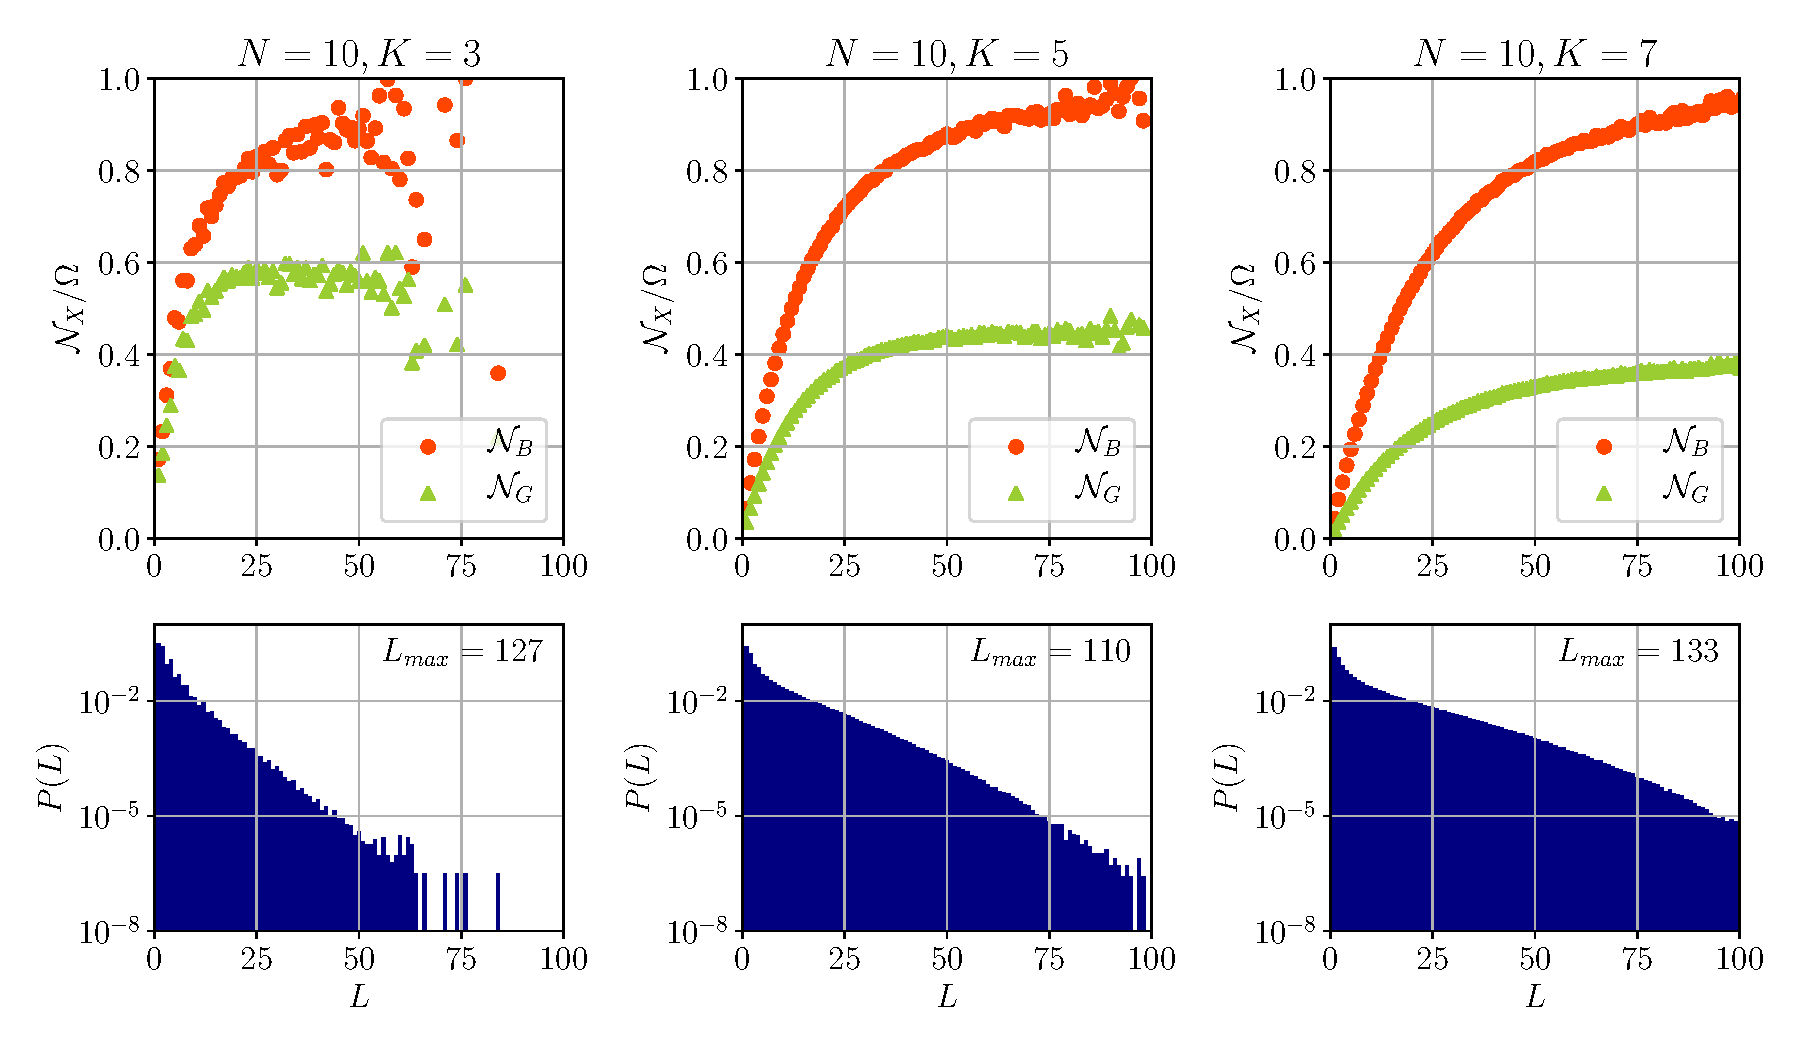
\includegraphics[width=\textwidth]{Plots/basin_sizes_N10_chaotic}
	\end{subfigure}
	\caption{Here we see plots like in Figure \ref{fig:basin_sizes_main}, only now for the in-degrees $K\in \{1,1.3,1.7\}$ (frozen) and $K\in \{3,5,7\}$ (chaotic). All were done over $10^6$ realizations. The upper plots show the averaged normalized basins of attraction (orange) and the part that the garden-of-Eden states (green) take up from the whole phase space. Below them we have the probability distribution for attractors with length L to appear.}
	\label{fig:basin_sizes_main_additional_frozen_chaotic}
\end{figure}
\newpage
\paragraph*{}\paragraph*{}\paragraph*{}
\section{Additional Plots to Figure \hyperref[fig:basin_hists]{3.11}}\label{sec:basin_hists_additional}
\begin{figure}[h!]
	\begin{subfigure}{\textwidth}
		\includegraphics[width=\textwidth]{Plots/basin_hists_N7_2}
	\end{subfigure}
	\begin{subfigure}{\textwidth}
		\includegraphics[width=\textwidth]{Plots/basin_hists_N9_2}
	\end{subfigure}
	\caption{Those plots are the histograms from Figure \ref{fig:basin_hists} with system sizes $N=7$ and $N=9$.}
	\label{fig:basin_hists_additional_sizes}
\end{figure}

\begin{figure}[h!]
	\begin{subfigure}{\textwidth}
		\includegraphics[width=\textwidth]{Plots/basin_hists_N8_3}
	\end{subfigure}
	\begin{subfigure}{\textwidth}
		\includegraphics[width=\textwidth]{Plots/basin_hists_N8_4}
	\end{subfigure}
	\caption{Those plots are the histograms from Figure \ref{fig:basin_hists} with system size $N=8$ with the numbers of attractors $N_A=3$ and $N_A=4$.}
	\label{fig:basin_hists_additional_attractors}
\end{figure}

\newpage
\paragraph*{}\paragraph*{}
\section{Additional Plots to Figure \hyperref[fig:single_flip_stability]{3.13}}
\begin{figure}[h!]
	\begin{subfigure}{\textwidth}
		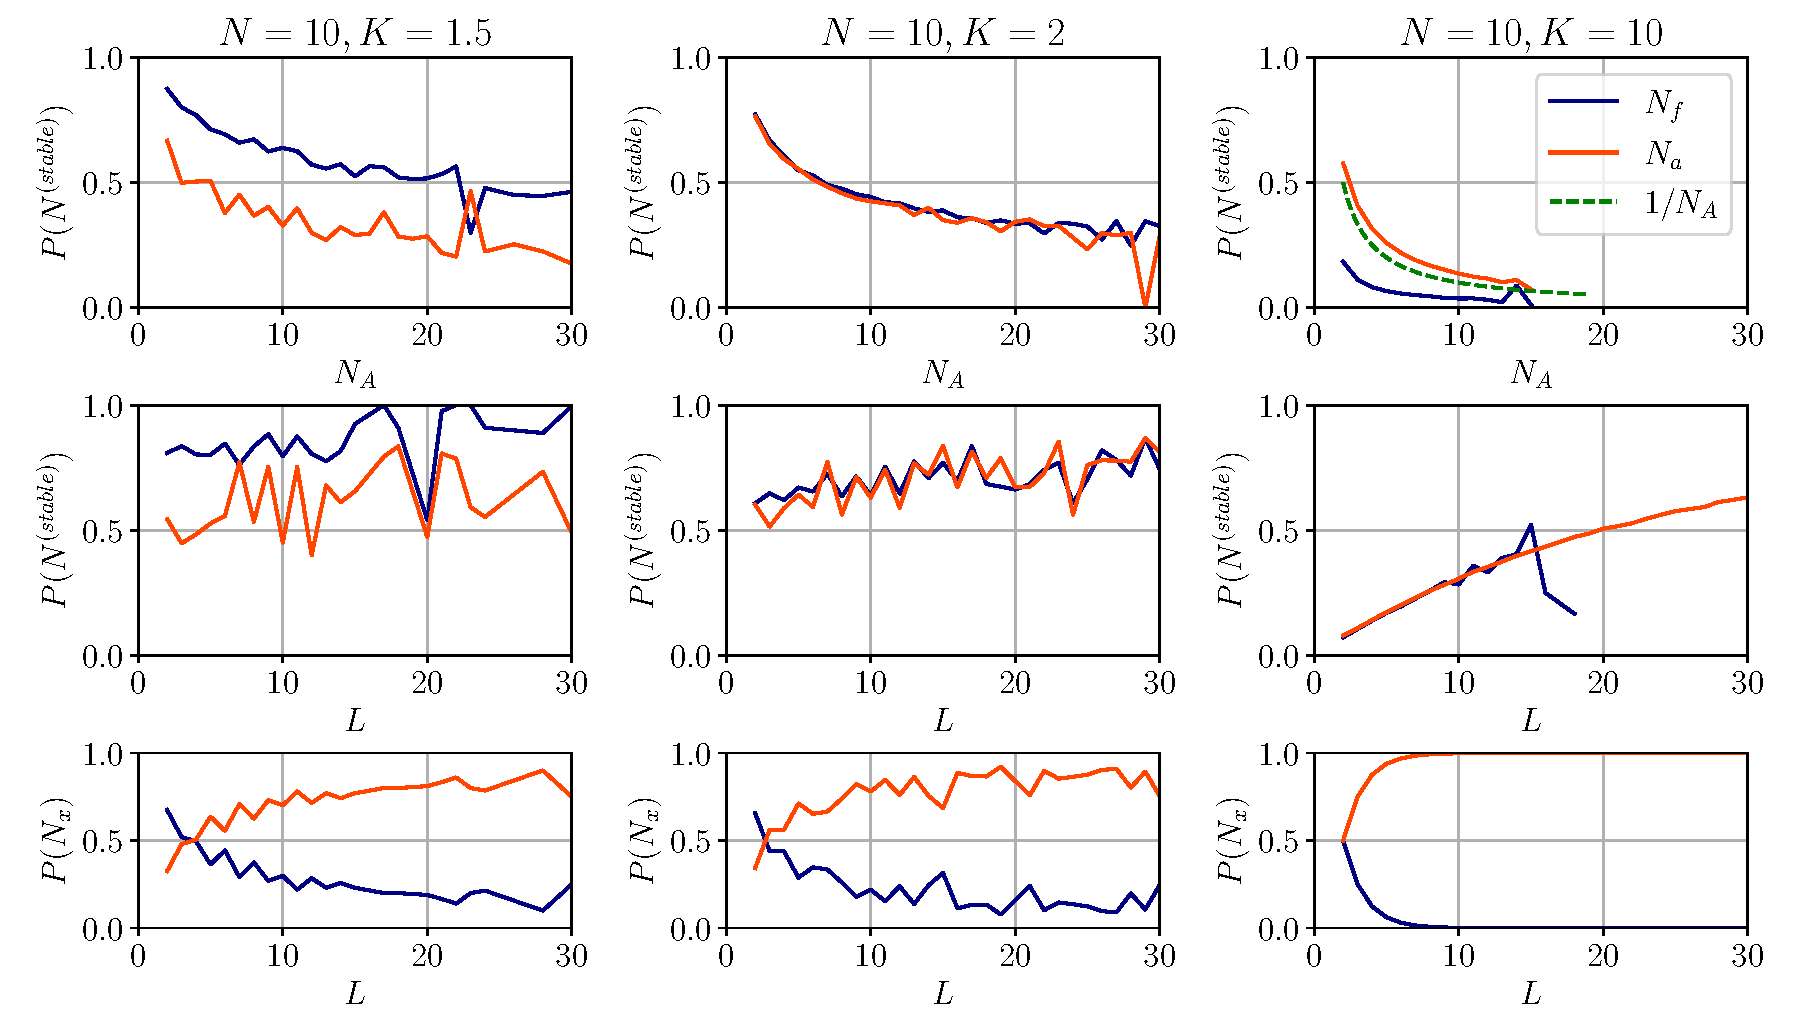
\includegraphics[width=\textwidth]{Plots/single_flip_stability_N10}
	\end{subfigure}
	\begin{subfigure}{\textwidth}
		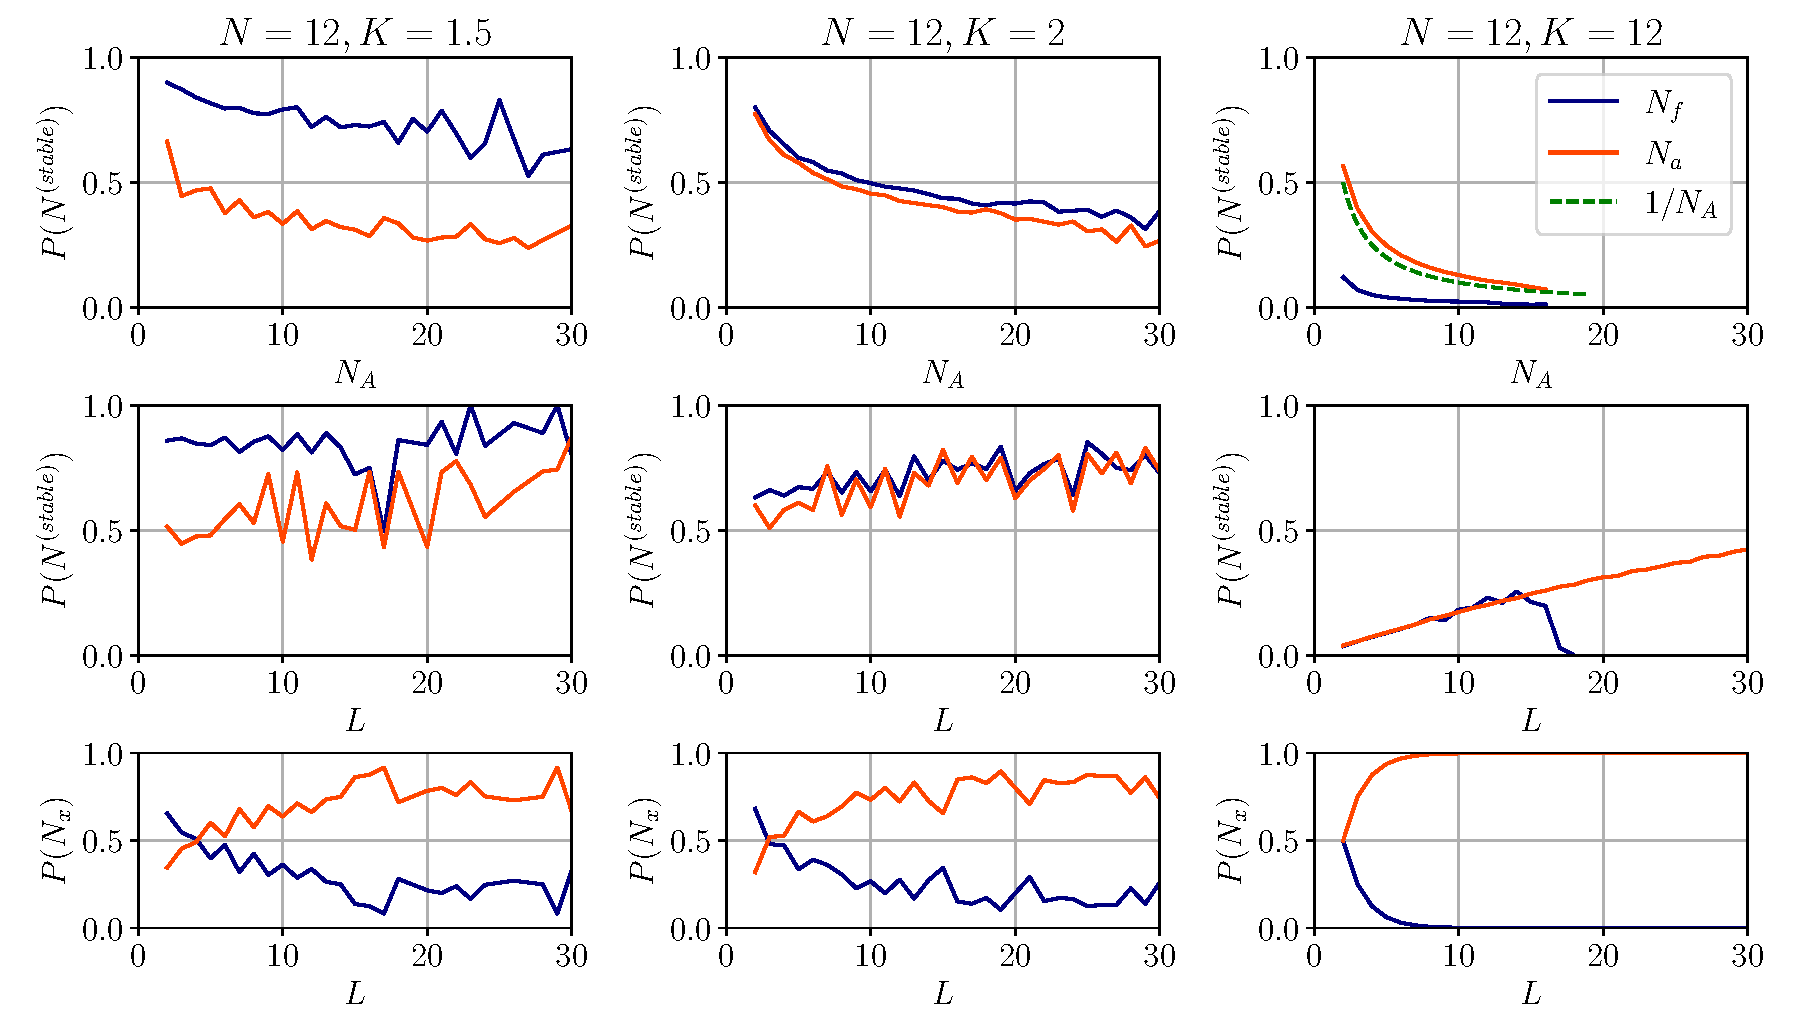
\includegraphics[width=\textwidth]{Plots/single_flip_stability_N12}
	\end{subfigure}
	\caption{Those plots show the graphs of stability like in Figure \ref{fig:single_flip} with system sizes $N=10$ and $N=12$. We compare the stability of frozen $ N_f $ and active nodes $ N_a $. As we have seen before, the critical networks are where both groups of nodes are equally stable independent of the network size.}
	\label{fig:single_flip_additional}
\end{figure}

